\newcommand{\pbArrow}{\,\leftrightarrow\,}

\newcommand{\xTwo}{\ensuremath{\tau}}

\newcommand{\xOne}[1]{\ensuremath{#1}}
\newcommand{\ta}[1]{\ensuremath{\xTwo_{#1}}}

\newcommand{\te}{\ensuremath{\ta{x}} }
\newcommand{\ex}{\ensuremath{\xOne{x}}}

\newcommand{\st}[1]{\ensuremath{\mathbf{#1}}}
\newcommand{\xst}{\ensuremath{\st{x}}}

\newcommand{\Hom}[1]{\ensuremath{\bar{#1}}}

\newcommand{\s}{\ensuremath{\sigma}}
\newcommand{\stilde}{\ensuremath{\tilde{\s}}}
\newcommand{\shom}{\ensuremath{\Hom{\s}}}
\newcommand{\smin}{\ensuremath{\Sigma}}
\newcommand{\sminhom}{\ensuremath{\Hom{\smin}}}
\newcommand{\snull}{\ensuremath{\sminhom_0}}

\newcommand{\ds}{\ensuremath{\delta \s}}
\newcommand{\dsx}[1]{\ensuremath{\ds(#1)}}
\newcommand{\dst}{\ensuremath{\delta \stilde}}
\newcommand{\dstx}[1]{\ensuremath{\dst(#1)}}

\newcommand{\qs}{\ensuremath{q_{\smin}}}
\renewcommand{\S}{\mathcal{S}}
\newcommand{\seff}{\mathcal{S}_{\text{eff}}}
\newcommand{\Z}{\ensuremath{\mathds{Z}}}
\newcommand{\gp}{\ensuremath{U}}
\newcommand{\gphom}{\ensuremath{\Hom{\gp}}}
\newcommand{\coupling}{\ensuremath{g^2}}
\newcommand{\rscoupling}{\ensuremath{g^2}}
\newcommand{\grandp}{\ensuremath{\Omega}}
\newcommand{\grandphom}{\ensuremath{\Hom{\grandp}}}

\newcommand{\energy}[1]{\ensuremath{E_{#1}}}

\newcommand{\gch}{\ensuremath{\gamma^\mathrm{ch}}}
\newcommand{\dop}{\ensuremath{D}}
\newcommand{\dophom}{\ensuremath{\Hom{\dop}}}

\newcommand{\gtwo}{\ensuremath{\Gamma^{(2)}}}
\newcommand{\gtwovar}[4]{\ensuremath{\gtwo ( #1, #2, #3, #4)}}
\newcommand{\gtwovardef}{\ensuremath{\gtwovar{\shom}{\mu}{T}{q}}}
\newcommand{\qmin}{\ensuremath{Q}}

\newcommand{\zwave}[3]{\ensuremath{Z ( #1, #2, #3 )}}

\section{Infinite-\texorpdfstring{$N$}{N} analysis of inhomogeneous phases}\label{sec:gnInfInhomo}
\begin{disclaimer}
	This section follows in large parts the discussion presented in \nbccite{Koenigstein:2021llr}.
	The plots of \nbccite{Koenigstein:2021llr} were produced by L. Pannullo.

	The following introduction of this section is based on Sec. I of \ccite{Koenigstein:2021llr}.
\end{disclaimer}

In this section we examine and cross-check the functionality of a stability analysis~\cite{\stabRefs} of a spatially homogeneous ground state and the closely related \acrrepeat{ggl} analysis~\cite{\gglRefs}, \cf{} our introductory remarks of \cref{subsec:inhomoMethods}.
Both present as very appealing indirect methods to study inhomogeneous phases without the need to explicitly compute with inhomogeneous condensates, thus avoiding the related major technical challenges commented on in \cref{subsec:inhomoMethods}.

Arguably the most prominent examples for spatially inhomogeneous condensation in relativistic \qfts{} are observed in \dimPlus{1}{1} dimensions.
In the \twoDimensional{} \gnm{} in \mf{} spatially oscillating condensates have been proven to be the true absolute ground states in some regions of the phase diagram~\cite{Brzoska:2001iq,Thies:2003kk,Thies:2003br,Schnetz:2004vr,Schnetz:2005ih,Schnetz:2005vh,Thies:2005wv,Thies:2006ti}, as already mentioned in our introduction of literature results in \cref{subsec:inhomoLiterature}.
In this section we will examine the results, shown and discussed around \cref{fig:GNthisPD} in detail.
In the \twoDimensional{} \gnm{} at infinite $N$ the exact spatial modulation of the inhomogeneous condensate was derived analytically in terms of known functions~\cite{Schnetz:2004vr,Schnetz:2005ih} deploying in parts semi-analytic techniques of supersymmetric quantum mechanics~\cite{Dunne:1997ia,Cooper:2001weo}.
Also more involved \twoDimensional{} models with more complicated symmetry breaking patterns exhibit an \gls{ip}~\cite{Schon:2000he,Schon:2000qy,Thies:2019ejd,Thies:2020ofv,Heinz:2015lua}.
For a general review regarding \glspl{ip} in the context of \hep{}, we refer again to \ccite{Buballa:2014tba} and our overview in the introduction of \cref{sec:inhomogeneousPhases}.

In \cref{subsec:inhomoMethods} we commented on the various direct and indirect methods to study inhomogeneous phases.
The stability analysis and the closely related \ggla{} as indirect methods are based on the idea  to determine the ground state assuming a spatially homogeneous condensate and to study position-dependent perturbations of this state in a second step.
Hence, one expands the full quantum effective action in the \gls{ir} in powers of the perturbation in a functional series.
By inspecting the two-point function, which is basically the curvature of the action at its homogeneous minimum (the homogeneous ground state), one can classify stable and unstable directions in field space from the sign of the two-point function.
Thus, one is performing a functional curve sketching and searches for expansion points that are saddle-points of the action.
A non-trivial minimum of the two-point function at non-zero external spatial momentum $q$ signals the instability of the homogeneous phase against inhomogeneous condensation, since the ground state energy can be lowered by forming an inhomogeneous condensate with relative momentum $q$.
	
This relatively simple concept allows to examine a sufficient, but not necessary condition for an \gls{ip}, \ie{}, if the homogeneous ground state is unstable \wrt{} inhomogeneous perturbations, the ground state must be inhomogeneous.
In simple terms, stability of the homogeneous condensate can be found, but the true global minimum of the action can still be an inhomogeneous field configuration located outside the range of validity of the stability analysis around the homogeneous ground state \dash{} which is of course a limitation of this approach.
We discuss this limitation at length in \cref{subsubsec:phase_diagram_stability_analysis}.

The \ggla{} can be seen as a variant of the stability analysis since it is basically an expansion of the stability analysis in powers of the homogeneous condensate and external momentum $q$.
It manifests as a gradient expansion of the effective action and as such is more limited when it comes to qualitative and especially quantitative predictive power as we will discuss in \cref{subsec:GNggl}.\bigskip

Howsoever, the great advantage of theses techniques is, that they are basically applicable to all kinds of models and theories.
They work independent of the technical method and approximation that is used to compute the underlying ``expansion coefficients''.

For example, the stability analysis has been applied in mean-field studies of a broad range of models but is also used in \gls{frg} calculations or in the context of lattice field theory.
There are multiple studies, see, \eg{}, \ccite{deForcrand:2006zz,Wagner:2007he,Winstel:2019zfn,Nakano:2004cd,Abuki:2011pf,Abuki:2013pla,Tripolt:2017zgc,Buballa:2018hux,Buballa:2020nsi,Buballa:2020xaa, Pannullo:2021edr}, which are based on a stability analysis or directly related approaches.
	
To the best of our knowledge, there has not been a significant attempt to discuss the limitations and successes of these method in great detail using a fully-understood/solved model, where the exact solution is well-known.
Hence, our goal is to revisit the \twoDimensional{} \gls{gn} model, as it has been solved analytically in \ccite{Schnetz:2004vr,Schnetz:2005ih} with an exact solution for the ground state for all temperatures $T$ and chemical potentials $\mu$, and extend earlier ``stability analyses''\footnote{In these works the term ``almost degenerate perturbation theory (ADPT)'' is used instead of ``stability analysis''. However, the approach is quite similar.} within this and closely related models~\cite{Thies:2003kk,Boehmer:2008uq,Boehmer:2007ea,Thies:2019ejd} and the \ggla{} put forward in \ccite{Abuki:2011pf}.
In this sense the present discussion is in the spirit of \cref{chap:zeroONSU2}: we again use exact reference values (now be it much more involved ones than just mere integrals) to rigorously test and evaluate computational methods (now the stability and \ggla{} instead of the \frg{} in a \cfd{} formulation).
	
At this point we emphasize that the work discussed in this section is explicitly not about groundbreaking new results or a concept that is original to this work.
It is merely a recapitulation and combination of existing literature results in a form that is meant to allow for a keener insight into the quantitative and qualitative predictive power of the stability analysis and related \ggla{} as indirect methods to study inhomogeneous condensates.\bigskip

This section is structured as follows: 
In \cref{subsec:phenomenology}, we briefly recapitulate the phenomenology of the \gnm{} in the infinite-$N$ limit, \viz{} its inhomogeneous phase diagram at (non-)zero baryon densities and (non-)zero temperature.

In \cref{subsec:stability} we discuss the stability analysis.
First we introduce the formalism for the stability analysis of bosonic two-point functions \wrt{} inhomogeneous perturbations.
After this technical introduction we discuss explicit results for the renormalized \gnm{} at infinite $N$ in the subsequent subsubsections.
In \cref{subsubsec:momentum_structure} we discuss numerical results for the two-point function.
The results for the detection of inhomogeneous condensation in the phase diagram via the stability analysis are presented and compared to the analytical solution of the model in \cref{subsubsec:phase_diagram_stability_analysis}.
In two additional subsections, namely \cref{subsubsec:wavevector,subsubsec:wave-function renormalization}, we compare the dominant mode of the exact inhomogeneous condensate with the dominant wave vector from the stability analysis and further comment on the values of the bosonic wave-function renormalization and its implications.

In \cref{subsec:GNggl} we confront the results obtained with a \ggla{}~\cite{Abuki:2011pf} with the analytical solution of the model.

\subsection{The inhomogeneous phase diagram of the Gross-Neveu model}
\label{subsec:phenomenology}
The inhomogeneous phase diagram of the \gls{gn} model for $N \to \infty$ is well-known, which makes it an ideal testing ground for methods in \glspl{qft}.
Therefore, we will briefly summarize the established phenomenology of the \gls{gn} in the $\mu$-$T$-plane as benchmark and reference values.
\fullWidthTwoColumnFigures%
	[!t] % Placement
	{%
		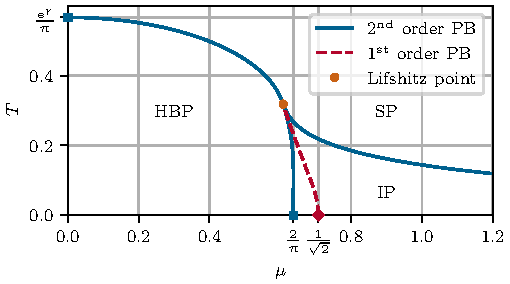
\includegraphics[width=\subcaptionFigureWidth]{gn/figures/largeN_pd.pdf} % left figure
		\captionsetup{width=\subcaptionFigureWidth}%
		\caption{%
			The phase diagram of the \gls{gn} model in the infinite-$N$ limit. The dashed red curve corresponds to the first-order phase boundary that is obtained if spatially homogeneous condensation is assumed~\cite{Wolff:1985av,Schon:2000qy}.
				The solid blue lines correspond to second-order phase transitions, if spatially inhomogeneous condensation is taken into account~\cite{Schnetz:2004vr,Schnetz:2005ih,Schnetz:2005vh,Basar:2009fg}.
			\fromFig{1}{Koenigstein:2021llr}
		}
		\label{fig:analytical_pd}
	}
	{\fullWidthTwoColumnFigureSpacing}
	{%
		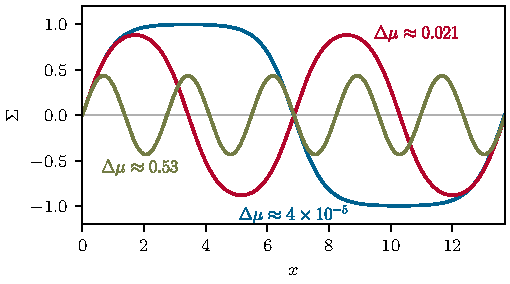
\includegraphics[width=\subcaptionFigureWidth]{gn/figures/condensate.pdf} % Right figure
		\captionsetup{width=\subcaptionFigureWidth}%
		\caption{%
			Spatial inhomogeneous chiral condensate $\smin ( \mu, T, \ex )$ at ${T = 0}$ for various chemical potentials $\mu$ with ${{\Delta\mu = ( \mu - \mu_c )/\snull}}$ in the \gls{ip} (where ${\mu_c/\snull = 2/\uppi}$).
				The curves are calculated using expressions of \ccite{Thies:2003kk,Schnetz:2004vr,Schnetz:2005ih}.
				This figure is inspired by Fig.~2 of \ccite{Thies:2003kk}.
			\fromFig{2}{Koenigstein:2021llr}
		}%
		\label{fig:inhomogeneous_condensate}
		%\vspace{1cm}
	}%

For related (and more comprehensive) discussions and original works of the rich large-$N$ phenomenology and physics of the \gls{gn} model we refer to \ccite{Jacobs:1974ys,Dashen:1974xz,Harrington:1974te,Harrington:1974tf,Dashen:1975xh,Affleck:1981bn,Cohen:1981qz,Cohen:1983nr,Wetzel:1984nw,Shankar:1985zc,Wolff:1985av,Karsch:1986hm,Treml:1989,Rosenstein:1990nm,Gracey:1990sx,Gracey:1990wi,Gracey:1991vy,Pausch:1991ee,Chodos:1993mf,Barducci:1994cb,Schon:2000he,Schon:2000qy,Brzoska:2001iq,Blaizot:2002nh,Thies:2003br,Thies:2003kk,Thies:2003zr,Schnetz:2004vr,Thies:2005vq,Schnetz:2005ih,Thies:2005wv,Schnetz:2005ih,Schnetz:2005vh,deForcrand:2006zz,Thies:2006ti,Karbstein:2006er,Boehmer:2007ea,Karbstein:2007be,Karbstein:2007bg,Wagner:2007he,Basar:2008im,Boehmer:2008uq,Basar:2009fg,Brendel:2009pq,Zinn-Justin:2010,Fitzner:2010nv,Dunne:2011wu,Fitzner:2012gg,Fitzner:2012kb,Dunne:2013rka,Thies:2014ida,Heinz:2015lua,Thies:2017mbl,Ahmed:2018tcs,Bermudez:2018eyh,Narayanan:2020uqt,Roose:2020znu,Quinto:2021lqn,lopes2021excitonic}.
	
Enforcing the ground state (the $\langle\Fpsib\Fpsi\rangle$-condensate) of the auxiliary field to be constant (homogeneous) in space-time, thus ${\s(x ) = \shom = \mathrm{const.}}$, we are in the setting of the previous \cref{sec:gnInfHomo}, where we discussed the homogeneous phase diagram~\ref{fig:GNlargeN_PD} at length in \cref{subsec:phase_diagram_mean_field}.
We recall the following findings in the language and notation\footnote{
In this subsection we denote the homogeneous condensate/fermion mass with $\sminhom ( \mu, T ) \equiv \sigma(\mu,T) h \equiv \Delta(\mu,T)$ with its value in vacuum $\snull\equiv \sminhom ( 0, 0 )\equiv\sigma(0,0) h \equiv\sigma_0 h \equiv \Delta_0$. 
At this point I have to apologize for the wealth of different \dash{} but at least not contradictory \dash{} notations for the same quantities in this part of my thesis.
Since this chapter is based on published results~\cite{Stoll:2021ori,Koenigstein:2021llr} involving different collaborators, the notations of \ccite{Stoll:2021ori,Koenigstein:2021llr} are slightly different.
Unifying the notations would require changing the plot labels and legends, which I deemed too time consuming and cumbersome when it comes to referencing the figure sources.
} used in this section:
We find a \acrrepeat{hbp} with a condensate $\sminhom ( \mu, T ) \neq 0$ (broken $\Z_2$ symmetry) at small $\mu$ and $T$ and the \acrrepeat{sp} with ${\sminhom ( \mu, T ) = 0}$ with restored $\Z_2$ symmetry in the rest of the $\mu$-$T$-plane.
The phase transition is of second-order at ${( \mu, T_c )/\snull = ( 0, \eu^\upgamma/\uppi ) \simeq (0,0.567 )}$ and ranges from ${\mu = 0}$ to the \acrrepeat{cp} at $( \mu_{\mathrm{CP}}, T_{\mathrm{CP}} )/\snull \simeq ( 0.608, 0.318 )$.
At this point the phase transition becomes first-order and continues to lower temperatures until it finally terminates at ${( \mu_{c, \text{hom}}, T )/\snull = ( 1/\sqrt{2}, 0.0 ) \simeq ( 0.707, 0.0 )}$.\bigskip
	
Relaxing the restrictive assumption of homogeneous condensation and allowing for a spatially varying background field ${\MFphi=\MFEIphi =\sigma( x )}$, a modified phase diagram is obtained. Here, one finds an \acrrepeat{ip} where the ground state ${\smin ( \mu, T ) = \smin ( \mu, T, x )}$ is an oscillating function in space.
This phase emerges for temperatures $T < T_L \simeq 0.318\, \snull$ and moderate chemical potentials $\mu >  \mu_L \simeq 0.608 \, \snull$ and grows in $\mu$-direction for decreasing temperature, \cf{}\ \cref{fig:analytical_pd} and  \ccite{Thies:2003kk,Thies:2003br,Schnetz:2004vr,Schnetz:2005ih,Schnetz:2005vh,Thies:2006ti}.
The former homogeneous first-order phase boundary is completely engulfed by the \gls{ip}.
The novel phase transition between the \gls{ip} and the \gls{hbp} is of second-order and ranges from ${( \mu_{c}, T )/\snull = ( 2/\uppi, 0. 0 ) \simeq ( 0.637, 0.0 )}$ to a \gls{lp} which is located at the position $( \mu_L, T_L )/\snull \simeq ( 0.608, 0.318 )$ of the former \gls{cp}. At the \gls{lp} three phases \dash{} a homogeneously broken, an inhomogeneously broken, and a restored phase \dash{} meet.
	
At the \gls{hbp}$\pbArrow$\gls{ip} phase boundary, the phase transition is not linked to the $\Z_2$ symmetry breaking/restoration, but rather to the breaking/restoration of spatial translational invariance, because discrete chiral symmetry is always (periodically) broken by the condensate.
The other phase boundary from the  \gls{ip} to the \gls{sp} is also of second-order and thus all phase boundaries of the \emph{correct}/\emph{revised} mean-field phase diagram correspond to second-order phase transitions.
Crossing the \gls{sp}$\pbArrow$\gls{ip} phase boundary the discrete chiral symmetry as well as spatial translational invariance are broken/restored.
This crucial difference between discrete chiral symmetry and translational invariance breaking/restoration is of great importance for the remainder of this work and the limitations of the stability analysis.
	
The spatially inhomogeneous chiral condensate in the \gls{ip} is described by Jacobi elliptic functions\footnote{For definitions, properties, and relations of the involved Jacobi elliptic functions, see, \eg{}, Chap.~22 of \ccite{NIST:DLMF}.}
\begin{align}
\smin = M_0 \sqrt{\nu}\, \mathrm{sn}(M_0 \vts x,\nu)\,,
\label{eq:Msn}
\end{align}
and for increasing chemical potential 
\begin{itemize}
	\item its shape evolves from a kink-antikink shape $(\nu\rightarrow 1)$ to a sine-like shape  $(\nu\rightarrow 0)$,
	
	\item its amplitude $M_0\sqrt{\nu}$ decreases \dash{} mainly due to the aforementioned decrease of $\nu$,
	
	\item its wave vector $q=\frac{2\piu}{M_0 \mathrm{K}(\nu)}$ increases,
\end{itemize}
as shown in \cref{fig:inhomogeneous_condensate} for zero temperature, see also \ccite{Schnetz:2004vr,Schnetz:2005ih}.
The general behavior of the condensate is very similar at non-zero temperature, see \ccite{Schnetz:2004vr} for details.

\subsection{Stability analysis of the spatially homogeneous \texorpdfstring{$\Z_2$}{Z2}-symmetric phase}\label{subsec:stability} 
\begin{disclaimer}
	This subsection is based on Sec.~II.D of \nbccite{Koenigstein:2021llr}.
	The four included subsubsections closely follow the discussions of Secs.~III.A\dash{}D of \ccite{Koenigstein:2021llr}.
	
	The numerical results for the stability analysis in the $\mu$-$T$-plane, \cf{} \cref{fig:pd_stability,fig:stability_wavevector_vs_condensate_wavevector_mu_T}, were obtained with my \Cpp{} code~\cite{Steil:2023GNcpp}, computing 49875 points in the $\mu$-$T$-plane in about two hours CPU time on an \ryzen{} processor (14 minutes wall time on 12 cores).
	The references values discussed in \cref{subsec:phenomenology}, see also \cref{fig:analytical_pd}, were computed by L. Pannullo in a few hours of wall time.	
\end{disclaimer}

In this subsection we turn to the theoretical considerations behind the stability analysis to detect spatially inhomogeneous phases and discuss numerical results in the following \cref{subsubsec:momentum_structure,subsubsec:phase_diagram_stability_analysis,subsubsec:wavevector,subsubsec:wave-function renormalization}, where we confront the results obtained from the stability analysis with the reference values discussed in \cref{subsec:phenomenology}.
The following discussion is in parts based on \ccite{Rechenberger:2018talk}, but similar discussions can be found in \ccite{Carignano:2019ivp,Buballa:2020nsi,Nakano:2004cd,Buballa:2018hux}.
We further deviate a bit from the presentation chosen in \ccite{Koenigstein:2021llr}, since we consider a computation of the homogeneous effective potential and the bosonic two-point function using the \frg{} framework.\bigskip

In order to relax the assumption of spatially homogeneous condensation and to search for a spatially \gls{ip}, one has to find the global $\ex$-dependent minima $\Sigma ( \mu, T, \ex )$ of the functional $\Gamma [ \sigma ( \ex ) ]$ for all possible field configurations $\sigma ( \ex )$.
Generically \dash{} as was already discussed in \cref{sec:inhomogeneousPhases} \dash{} this is an extremely challenging task, both analytically and numerically.

Due to these challenges, the idea of an indirect detection of inhomogeneous condensation arose, which is based on analyzing the stability of the spatially homogeneous ground state against inhomogeneous perturbations.
This was already discussed and/or applied in various contexts~\cite{Fu:2019hdw,Winstel:2021yok,Buballa:2020nsi,Winstel:2019zfn,Buballa:2018hux} and to some extent also in the context of the (chiral) \gls{gn} model~\cite{Thies:2003kk,Thies:2019ejd}.
The proposed approach allows to search for a sufficient condition for an \gls{ip}, \ie{}, if $\sminhom ( \mu, T )$ is unstable against spatially inhomogeneous perturbation, the true ground state has to be inhomogeneous.
In general, $\sminhom ( \mu, T )$ could, however, be stable against inhomogeneous perturbations, but by a functional minimization of $\Gamma [\sigma ( \ex ) ]$ one may still find an inhomogeneous ground state.
In this scenario the local, homogeneous and the global, inhomogeneous minimum are separated by a ``potential barrier'', which prevents a stability analysis and calls for global minimization approaches.
This implies that the stability analysis is expected to work properly in the vicinity of second-order phase boundaries between homogeneous and inhomogeneous phases.
Nonetheless, this model and approximation independent method is still a powerful tool for the search of exotic phases of matter.
Note that the construction/expansion is technically not limited to the trivial homogeneous minimum $\sminhom ( \mu, T )=0$. \bigskip

On a formal level the stability analysis is based on a functional (Taylor) expansion of the effective action ${\Gamma [ \s ]}$ about a spatially homogeneous background field $\shom$ in powers of an inhomogeneous perturbation $\dsx{\ex}$.
A spatially homogeneous ground state is considered to be unstable, if the second-order coefficient of this expansion exhibits some unstable direction in field space, if it is evaluated on the spatially homogeneous minimum $\sminhom ( \mu, T )$.
Note that the first-order coefficient in this expansion vanishes due to the \qeom{} \cref{eq:QEOM} when evaluated on the \ir{} minimum $\sminhom ( \mu, T )$.
On a mean-field/large-$N$ level this is encoded by the homogeneous gap \cref{eq:gapeq}.

The second-order Taylor coefficient is the bosonic two-point function $\gtwo$, which is analyzed in momentum space.
An unstable direction in field space corresponds to a negative value $\gtwo$ for external spatial momentum $q$, which can be associated to the wave vector of a spatially oscillating energetically preferred ground state.
This implies a lower ground state energy for the inhomogeneous phase when compared to the homogeneous one assuming the higher-order contributions of the expansion beyond the second-order are either positive or negligible.
Whether or not this assumptions are met depends on the model, the expansion point and the magnitude of the inhomogeneous oscillations as we will discuss in detail in the following.
Hence, the stability analysis corresponds to searching for a sign change in $\gtwo$ at some external momentum $q$ in the $\mu$-$T$-plane.

\Ccite{Koenigstein:2021llr} includes a derivation of this two-point function and the corresponding expansion of ${\Gamma [ \s ]}$ in a conventional mean-field/large-$N$ setting~\cite{Carignano:2019ivp,Buballa:2020nsi,Nakano:2004cd,Buballa:2018hux} using the effective classical action $\seff [ \s ]$.
For details using this approach we refer to the corresponding discussion in Sec.~II.D of \nbccite{Koenigstein:2021llr}. 
We are in this work in the comfortable position that we have the \frg{} at our disposal which allows us to compute \nptFunctions{} \dash{} including the bosonic two-point function required for the following discussion.
We have introduced the flow equations for higher-order \nptFunctions{} in \cref{subsec:higherOrderFlowEquations} and have already encountered flow equations for two-point functions in the context of our zero-dimensional $SU(2)$ model, \cf{} \cref{paragraph:0dSU2flowmY}.
Details for the computation of the bosonic two-point function in the limit $N\rightarrow \infty$ can be found in \cref{app:GNtwopt}.
It should also be noted that in the renormalized limit $\Lambda\rightarrow \infty$ results of (fermionic) one-loop computations are in general completely regularization-scheme-independent.
At this point we just want to give the result of the computations outlined in \cref{app:GNtwopt}, \viz{} the bosonic two-point function for the \gnm{} in the renormalized limit at infinite $N$:
\begin{align}
	\gtwovardef &=\tfrac{1}{2\uppi} \ln \Big( \frac{\shom^2}{\snull^2} \Big)  - \ell_2 ( \shom, \mu, T, q )\,+\notag\\[.2em]
		&\qquad\qquad+\frac{1}{\uppi}\int_{0}^{\infty} \dif p \, \frac{1}{\energy{p}} \, ( \nf (\beta[\energy{p}+\mu]) + \nf(\beta[\energy{p}-\mu]) )\, ,	\label{eq:gtwo_renorm}
\end{align}
with the energies ${{\energy{p} = \sqrt{p^2 + \shom^2}}}$ and the integral
\begin{align}
	\ell_2 ( \shom, \mu, T, q ) = \, & - \Big( \frac{q^2}{2} + \shom^2 \Big) \, \frac{2}{\uppi} \int_{0}^{\infty} \dif p \, \frac{1}{\energy{p}} \, \Big( \frac{1}{\energy{p + q}^2 - \energy{p}^2} + \frac{1}{\energy{p - q}^2 - \energy{p}^2} \Big) \, \times \notag\\[.2em] 
	&\qquad\qquad\qquad\qquad\qquad \times\Big( 1 -\nf (\beta[ \energy{p}+\mu] ) - \nf (\beta[\energy{p} - \mu] )\Big) \, .	\label{eq:ell2}
\end{align}
The result \cref{eq:gtwo_renorm} can be further simplified, if at least one of the four arguments $\shom$, $\mu$, $T$, or $q$ is zero.
All possible cases and the respective simplifications of $\gtwo$ are listed in Tab.~I of \nbccite{Koenigstein:2021llr} with corresponding symbolic expressions in App.~A of \nbccite{Koenigstein:2021llr}.
A detailed derivation and discussion of the different cases is presented in \ccite{Koenigstein:2022phd}.

Negative values of $\gtwovar{\sminhom ( \mu, T )}{\mu}{T}{q}$ indicate an instability of the homogeneous minimum $\sminhom ( \mu, T )$ \wrt{}  inhomogeneous perturbations of momentum $q$.
Consequently, the two-point function can be used to search for inhomogeneous ground states for arbitrary $\mu$ and $T$.
This can be done by analyzing $\gtwovar{\sminhom ( \mu, T )}{\mu}{T}{q}$ as a function of $q$ for each point $( \mu, T )$ in the phase diagram.
In practice one searches for regions where $\gtwo(q)$ is negative.

\paragraph{The wave-function renormalization}\phantomsection\label{paragraph:GNZphi}\mbox{}\\%
In the past it was speculated, if it might be sufficient to study the curvature of $\gtwovar{\sminhom ( \mu, T )}{\mu}{T}{q}$ at ${q = 0}$, \ie{}, the second-order coefficient of a Taylor expansion of the two-point function in momentum space about ${q=0}$, \viz{} the wave-function renormalization,
\begin{equation}
	\zwave{\shom}{\mu}{T} \equiv \frac{1}{2} \frac{\dif^{\, 2}}{\dif q^2} \gtwovardef \Big|_{q = 0} \, .	\label{eq:wave-function_renormalization_definition}
\end{equation}
It was speculated that a negative bosonic wave-function renormalization might be sufficient to destabilize spatially homogeneous ground states and to energetically favor gradients in the spatial profile of the ground state over a spatially uniform ground state field configuration.
	
As pointed out, \eg{}, in \ccite{Roscher:2015xha,Fu:2019hdw}, a negative wave-function renormalization is only indicative towards the possibility for spatial modulations of the ground state.
It is not a sufficient or even necessary criterion, because higher-order momentum-dependencies of the bosonic two-point function might again disfavor spatially inhomogeneous condensation over homogeneous condensation.
Consequently, a study of the full momentum structure of the two-point function is necessary.
	
Nevertheless, the wave-function renormalization is still an extremely important quantity, as it directly enters the dispersion relations~\cite{Pisarski:2021qof,Rennecke:2021ovl}, see also our discussion in \cref{paragraph:GNbGNGNY}.
Explicit expressions for $\zwave{\shom}{\mu}{T}$, where $\shom$, $\mu$, and $T$ take either non-vanishing or vanishing values, can be found in App.~B of \nbccite{Koenigstein:2021llr} with an overview in table II of the aforementioned publication.
The physically relevant wave-function renormalization is again obtained, if \cref{eq:wave-function_renormalization_definition} is ultimately evaluated at the homogeneous ground state ${\shom = \smin ( \mu, T )}$.

Finally, we turn to the actual results and the promised proof of concept.
We start in \cref{subsubsec:momentum_structure} by presenting the $q$-dependence of the bosonic two-point function at various points in the $\mu$-$T$-plane.
The discussion of this momentum structure provides deeper insights in the (physical pairing) mechanisms and the operating principle behind the stability analysis.
Furthermore, we come back to these results, when we comment on recent calculations in the \gls{gn} model beyond the mean-field approximation~\cite{Pannullo:2019bfn,Pannullo:2019prx,Lenz:2020bxk,Lenz:2020cuv} including implications for our research in the next \cref{sec:gnyFiniteN}.
Based on the analysis in  \cref{subsubsec:momentum_structure} the actual stability analysis of the homogeneous phase in the $\mu$-$T$-plane can be performed and results are presented in \cref{subsubsec:phase_diagram_stability_analysis}.
Here, we demonstrate that this method is actually able to detect the well-known second-order phase-transition line between the \gls{ip} and the \gls{sp}, but also comment on its shortcomings.
Afterwards in \cref{subsubsec:wavevector}, the momentum profile of the bosonic two-point function, \ie{}, the dominant wave vector, is compared with the analytic solutions \eqref{eq:Msn} from \ccite{Schnetz:2004vr}.
Finally, we close the discussion of our results by presenting results for bosonic wave-function renormalization in the $\mu$-$T$-plane in \cref{subsubsec:wave-function renormalization}.
We again comment on the insufficiency of the wave-function renormalization as a single measure for the detection of spatially inhomogeneous condensates. Furthermore, we discuss possible implications on the quality of the mean-field approximation based on our quantitative calculations.

\subsubsection{The momentum structure of the bosonic two-point function}
\label{subsubsec:momentum_structure}
\fullWidthTwoColumnFigures%
	[!t] % Placement
	{%
		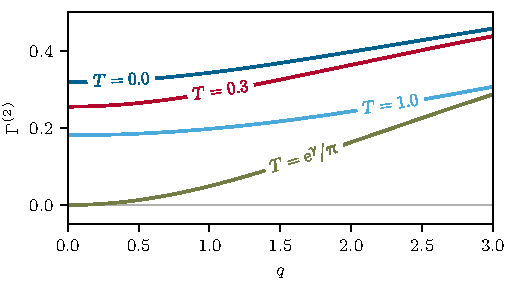
\includegraphics[width=\subcaptionFigureWidth+0.1cm]{gn/figures/gamma2_compare_0.pdf} % left figure
		\captionsetup{width=\subcaptionFigureWidth}%
		\caption{%
			The bosonic two-point function $\gtwovar{\shom}{\mu}{T}{q}$ as a function of the external momentum $q$ at vanishing chemical potential ${\mu = 0}$ and fixed temperatures ${T/\snull \in \{ 0.0, 0.3, \eu^\upgamma / \uppi , 1.0 \}}$ evaluated at the respective homogeneous minimum ${\shom = \sminhom ( \mu, T )}$.
			\fromFig{3}{Koenigstein:2021llr}
		}
		\label{fig:gamma2_compare_0}
	}
	{\fullWidthTwoColumnFigureSpacing}
	{%
		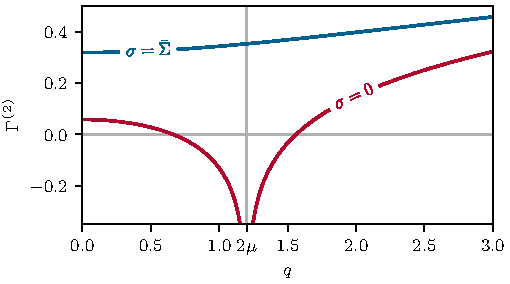
\includegraphics[width=\subcaptionFigureWidth-0.1cm]{gn/figures/gamma2_compare_1.pdf} % Right figure
		\captionsetup{width=\subcaptionFigureWidth}%
		\caption{%
			The bosonic two-point function $\gtwovar{\shom}{\mu}{T}{q}$ as a function of the external momentum $q$ at constant chemical potential ${\mu/\snull = 0.6}$ and vanishing temperature ${T = 0}$ evaluated at the homogeneous global minimum ${\shom = \sminhom ( \mu, 0 ) \neq 0}$ and the homogeneous local minimum ${\shom = 0}$.
			The unphysical red curve (stemming from an evaluation away from the homogeneous ground state, \viz{} ${\shom = 0}$) has a pole at ${q = 2\mkern2mu \mu}$.
			\fromFig{4}{Koenigstein:2021llr}
		}%
		\label{fig:gamma2_compare_1}
		%\vspace{1cm}
	}%
The entire idea of the stability analysis is based on the momentum structure/dispersion of the bosonic two-point function \eqref{eq:gtwo_renorm}.
Therefore, this subsubsection contains a detailed discussion of the various possible shapes of $\gtwo$, which occur in the \gnm{} at different points $( \mu, T )$ in the phase diagram.
Our discussion is based on \cref{fig:gamma2_compare_0,fig:gamma2_compare_1,fig:gamma2_compare_2,fig:gamma2_compare_3,fig:gamma2_sigma_q}, which were directly produced by (numeric) evaluation of \cref{eq:gtwo_renorm} or its simplified versions, see Tab.~I and App.~A of \nbccite{Koenigstein:2021llr}.
If needed, the corresponding spatially homogeneous ground state $\sminhom ( \mu, T )$ was determined (numerically) by minimization of \cref{eq:rg-U-MF-largeLambda}.\bigskip

We begin our discussion at vanishing chemical potential ${\mu = 0}$.
The corresponding plots for $\gtwovar{\sminhom ( 0, T )}{0}{T}{q}$ are presented in \cref{fig:gamma2_compare_0}.
One finds that the bosonic two-point function is always positive and convex for all external momenta at ${\mu = 0}$.
This is the case for zero and non-zero temperature, in the $\Z_2$ symmetry broken and symmetric phase respectively.
Consequently, the spatially homogeneous minimum is stable against inhomogeneous perturbations.
Furthermore, this might also imply that a low order derivative expansion of the bosonic effective action, \eg{}, in the context of the following computation at finite $N$ in \cref{sec:gnyFiniteN}, should be a decent approximation and capture the relevant momentum-dependencies.
Additionally, this confirms that it is unlikely to generate crystalline like ground states at zero density. 
Only at the phase transition at ${T/\snull = \eu^\upgamma/\uppi}$ the curve for $\gtwo$ has a single root at ${q = 0}$, which is expected, since the bosonic curvature mass vanishes at this phase transition~\cite{Dolan:1973qd,Weinberg:1974hy,Harrington:1974tf,Thies:2003kk}.\bigskip

Next, \cref{fig:gamma2_compare_1} is discussed, where we plot $\gtwovar{\shom}{\mu}{T}{q}$ at constant chemical potential ${\mu/\snull = 0.6}$ and vanishing temperature ${T = 0}$ for two evaluation points $\shom$ in the constant background field space.
As can be seen from \cref{fig:analytical_pd} this $\mu$-$T$-point lies in the \gls{hbp} implying that the true homogeneous ground state has ${\sminhom ( \mu, 0 ) \neq 0}$.
The two curves in \cref{fig:gamma2_compare_1} show that it is crucial to evaluate $\gtwovardef$ at the correct homogeneous minimum ${\shom = \sminhom ( \mu, 0 ) \neq 0}$ as the evaluation at ${\shom = 0}$ leads to negative values of $\gtwo$ giving a false signal of instability.
This seems somewhat obvious, especially for the rather simple \gls{gn} model in mean-field approximation.
However, for example in more involved \gls{frg} model calculations as in  \ccite{Eser:2018jqo,Eser:2019pvd,Cichutek:2020bli,Divotgey:2019xea,Tripolt:2017zgc,Pawlowski:2014zaa,Grossi:2021ksl,Otto:2019zjy,Otto:2020hoz,Dupuis:2020fhh,Eser:2021ivo} and especially for advanced truncations, it is sometimes not obvious to determine the correct evaluation point in field space for correlation functions \dash{} at least during the \rg{} flow.\bigskip

\fullWidthTwoColumnFigures%
	[!t] % Placement
	{%
		\vspace{.1cm}
		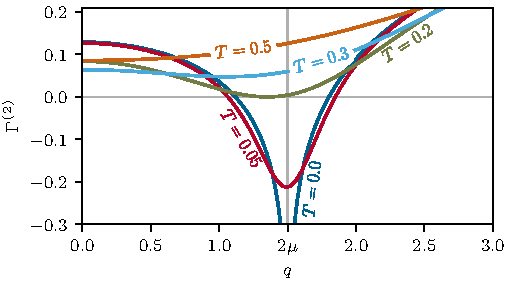
\includegraphics[width=\subcaptionFigureWidth-0.1cm]{gn/figures/gamma2_compare_2.pdf} % left figure
		\captionsetup{width=\subcaptionFigureWidth}%
		\caption{%
			The bosonic two-point function $\gtwovar{\shom}{\mu}{T}{q}$ as a function of the external momentum $q$ at constant chemical potential ${\mu/\snull = 0.75}$ and fixed temperatures ${T/\snull \in \{ 0.0, 0.05, 0.2, 0.3, 0.5 \}}$ evaluated at the respective homogeneous minimum ${\shom = \sminhom ( \mu, T )=0}$.
				The curve for ${T = 0.0}$ has a pole at ${q = 2 \, \mu}$, \textit{cf.} Eq.~(A15) of \ccite{Koenigstein:2021llr}.
			\fromFig{5}{Koenigstein:2021llr}
		}
		\label{fig:gamma2_compare_2}
	}
	{\fullWidthTwoColumnFigureSpacing}
	{%
		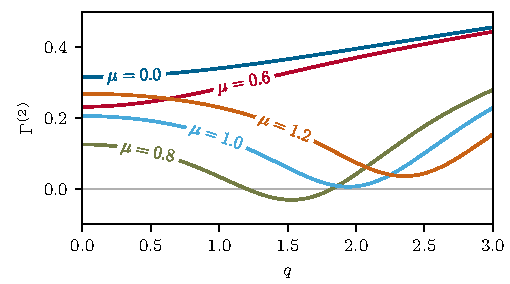
\includegraphics[width=\subcaptionFigureWidth+0.1cm]{gn/figures/gamma2_compare_3.pdf} % Right figure
		\captionsetup{width=\subcaptionFigureWidth}%
		\caption{%
			The bosonic two-point function $\gtwovar{\shom}{\mu}{T}{q}$ as a function of the external momentum $q$ at constant temperature ${T/\snull = 0.15}$ and fixed chemical potentials ${\mu/\snull \in \{ 0.0, 0.6, 0.8, 1.0, 1.2 \}}$ evaluated at the respective homogeneous minimum ${\shom = \sminhom ( \mu, T )}$.
			\fromFig{6}{Koenigstein:2021llr}
		}%
		\label{fig:gamma2_compare_3}
		%\vspace{1cm}
	}%
After covering the simple scenarios, we turn to \cref{fig:gamma2_compare_2}, where we plot the behavior of $\gtwo$ for different temperatures but constant chemical potential ${\mu/\snull = 0.75}$.
As discussed in \cref{subsec:phenomenology} and \cref{fig:analytical_pd}, these $\mu$-$T$-points are located in the \gls{sp} and in the \gls{ip}, such that the correct evaluation point in background field space is always the trivial homogeneous minimum ${\shom = \sminhom ( \mu, T ) = 0}$.
As expected we find a manifestly positive and convex $\gtwo$ at high temperatures, where thermal fluctuations are likely to vaporize any kind of crystal like structures and condensates, because the temperature $T$ and not the chemical potential $\mu$ is the dominating external energy scale.
On the other hand, for moderate temperatures one finds that $\gtwo$ develops a non-trivial minimum at some non-zero $q$, which indicates that the energy scale set by $\mu$ gains in importance.
However, this non-trivial minimum does not destabilize the spatially homogeneous ground state if $\gtwo$ stays manifestly positive.
Only below a certain threshold for the temperature (here $T/\snull \approx 0.2$), where the minimum of $\gtwo$ turns negative, an instability is observed implying a breaking of the $\Z_2$ symmetry and translational invariance by some lower lying ground state $\smin ( \mu, T, \ex )$.
Exactly at the temperature threshold the new $\ex$-dependent ground state $\smin ( \mu, T, \ex )$ is anticipated to exhibit a single wave vector $\qmin$, namely the single touching root of $\gtwo$.
The latter is equal to the minimum of the two-point function.
This is discussed in detail in \cref{subsubsec:wavevector}.
In the following, $\qmin$ generically denotes the location of the minimum of $\gtwo$ in $q$-direction, \ie{}, 
\begin{align}
	\label{eq:qmin}
	\qmin \equiv \mathrm{argmin}_q \, \gtwovar{\sminhom( \mu, T )}{\mu}{T}{q}\, .
\end{align}
Further decreasing the temperature, we observe in \cref{fig:gamma2_compare_2} that the $q$-range where $\gtwo$ is negative initially grows.
Additionally, the minimum of $\gtwo$ gets more and more negative and ultimately turns into a pole at ${q = 2 \, \mu}$ for ${T = 0}$.	
The roots of $\gtwo$ which are poles of the propagator $1/\gtwo$ signal a resonance in the respective anti-fermion-fermion two-point function $\langle\bar{\psi}\,\psi \rangle$. 
This resonance is associated with an anti-fermion-fermion bound state in which an anti-fermion and a fermion of opposite chirality are paired with a non-zero total momentum forming an inhomogeneous chiral condensate.
More details and qualitative as well as quantitative discussions of this pairing mechanism can be found in \ccite{Kojo:2009ha,Kojo:2011cn,Buballa:2014tba}.
The preferred momenta for the anti-fermion-fermion pairs are from the momentum range of negative $\gtwo(q)$ with the dominant frequency $Q$ typically associated with the minimum of $\gtwo$, see \cref{eq:qmin}.
The dominant frequency of $Q\sim 2\,\mu$ at low and especially zero temperature is typical for such inhomogeneous condensates as the anti-fermion-fermion pairs are formed in vicinity of the Fermi surface~\cite{Kojo:2009ha,Kojo:2011cn,Buballa:2014tba}.
Apart from the identification of the dominant frequency $Q$ the course of $\gtwo(q)$ for $\gtwo<0$ between the roots (including the pole at ${q=2\,\mu}$ for ${T=0}$) is not very instructive because the employed stability analysis using a homogeneous expansion point is incapable of capturing the full physics of the inhomogeneous chiral condensate in this momentum regime.
A notable exception occurs when we have a single touching root, in \cref{fig:gamma2_compare_2} the case for $T\approx0.2$, signaling the onset of instability of the homogeneous phase in favor of an inhomogeneous phase with an explicit single momentum mode $Q$ instead of a spectrum.
We will discuss this further in the following \cref{subsubsec:phase_diagram_stability_analysis}.\bigskip

Lastly, \cref{fig:gamma2_compare_3} is considered, where again $\gtwo$ is presented at different points in the phase diagram.
In contrast to the previous discussion, we do not vary the temperature at constant chemical potential, but fix ${T/\snull = 0.15}$ and study curves at various chemical potentials.
As can be seen from \cref{fig:analytical_pd} the slice through the phase diagram at ${T/\snull = 0.15}$ is chosen, because of its rich phenomenology at different $\mu$.
Starting from zero density at ${\mu = 0}$, a convex and manifestly positive function course of $\gtwo$ is observed.
Increasing $\mu$ the bosonic curvature mass (the value of $\gtwo$ at ${q = 0}$) is lowered, but $\gtwo$ stays convex.
As soon as one leaves the \gls{hbp} and crosses the first-order phase boundary to the $\Z_2$-symmetric phase (for spatially homogeneous condensates), \cf{}  \cref{fig:analytical_pd}, $\gtwo$ immediately develops a non-trivial negative minimum (for ${\mu/\snull = 0.8}$ at $q/\snull \approx 1.6$ in \cref{fig:gamma2_compare_3}), which indicates that spatially inhomogeneous condensation is energetically favorable and $\mu$ completely dominates the dynamics as an external energy scale, \ie{}, one enters the \gls{ip}.
However, further increasing $\mu$ at non-zero $T$ ultimately shifts the $\gtwo$-profile to larger values, such that at $\mu/\snull \approx 1.0$ the minimal value of $\gtwo$ turns positive again, see \cref{fig:gamma2_compare_3}.
This means that by further increasing $\mu$ we again cross a phase transition line and enter ultimately the $\Z_2$-symmetric and translation invariant phase.

At this point we remark, that the $q$-profiles for $\gtwo$ in \cref{fig:gamma2_compare_0,fig:gamma2_compare_1,fig:gamma2_compare_2,fig:gamma2_compare_3} are very similar to courses of $\gtwo$ that were sketched in Fig.~5 of \ccite{Roscher:2015xha} or the ones calculated and displayed in different contexts in Fig.~5 of \ccite{Tripolt:2017zgc}, Fig.~2 of \ccite{Buballa:2018hux}, and Fig.~8 of \ccite{Nakano:2004cd}.\bigskip

\fullWidthTwoColumnFigures%
	[!t] % Placement
	{%
		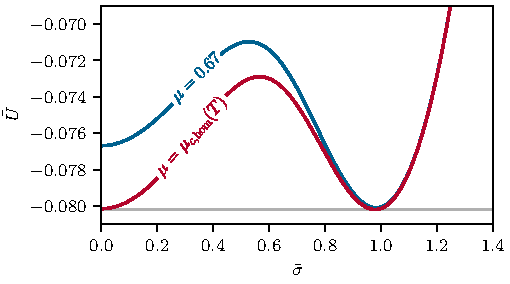
\includegraphics[width=\subcaptionFigureWidth]{gn/figures/ueff.pdf} % left figure
		\captionsetup{width=\subcaptionFigureWidth}%
		\caption{%
			The homogeneous effective potential $\gphom ( \shom, \mu, T )$  as a function of the homogeneous background field $\shom$ at constant temperature ${T/\snull = 0.1}$ and fixed chemical potentials $\mu/\snull \in \{ 0.67, \mu_{c,\text{hom}}(T)\}$, where $\mu_{c,\text{hom}}(T)\approx0.686$ is the critical chemical potential of the homogeneous phase transition at this temperature.
			\fromFig{7}{Koenigstein:2021llr}
		}
		\label{fig:ueff}
	}
	{\fullWidthTwoColumnFigureSpacing}
	{%
		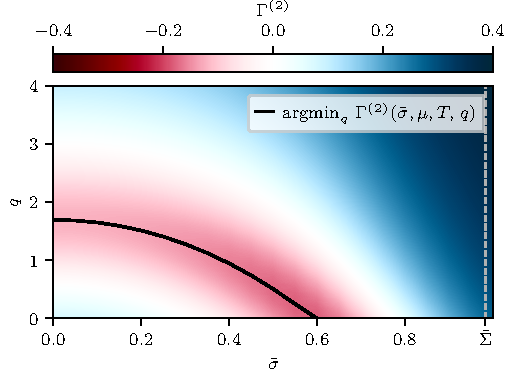
\includegraphics[width=\subcaptionFigureWidth]{gn/figures/gamma2_q_sigma.pdf} % Right figure
		\captionsetup{width=\subcaptionFigureWidth}%
		\caption{%
			The bosonic two-point function $\gtwovar{\shom}{\mu}{T}{q}$ in the $\shom$-$q$-plane for the point ${( \mu, T )/\snull = ( 0.67, 0.1 )}$ in the phase diagram.
			The solid black line marks the non-trivial minima.
			\fromFig{8}{Koenigstein:2021llr}
		}%
		\label{fig:gamma2_sigma_q}
		%\vspace{1cm}
	}%
	We conclude this subsubsection with a discussion of a shortcoming of the stability analysis.
To do so, a point in the phase diagram  is studied that is located extremely close to the first-order phase transition line in \cref{fig:analytical_pd}, but still only just corresponds to the \gls{hbp}, if only spatially homogeneous condensation is considered.
At ${( \mu, T )/\snull = ( 0.67, 0.1 )}$ the correct homogeneous minimum of the effective potential $\gphom$ is located at ${\bar{\sigma} = \sminhom/\snull \approx 1.0}$, while the point ${\shom = 0}$ corresponds to a local minimum, which is of similar depth, see \cref{fig:ueff}.

However, it is known from the exact solution~\cite{Schnetz:2004vr,Schnetz:2005ih,Schnetz:2005vh}, see \cref{fig:analytical_pd}, that this point in the $\mu$-$T$-plane actually corresponds to the \gls{ip}, if one allows for spatial modulations of the ground state.
For selected sample points we experienced during this subsubsection that the stability analysis seems to work well, if the expansion point is the trivial homogeneous minimum of the effective potential in the $\Z_2$-symmetric phase, thus ${\sminhom ( \mu, T ) = 0}$.
Naturally the question arises whether or not the stability analysis maintains its predictive power even with non-trivial spatially homogeneous expansion points $\sminhom ( \mu, T ) \neq 0$ are considered.
Hence, we present $\gtwovardef$ at ${( \mu, T )/\snull = ( 0.67, 0.1 )}$ as a function of $\shom$ and $q$ in \cref{fig:gamma2_sigma_q}.

Evaluating $\gtwo$ at large values of $\shom$, \eg{}, at the correct homogeneous minimum and expansion point $\sminhom/\snull \approx 1$, the bosonic two-point function is manifestly positive and does not signal any instability.
The reason is that the non-trivial homogeneous minimum and the spatially oscillating minimum are separated by a kind of ``potential barrier'', as the effective potential increases when studying small perturbations about the homogeneous minima.
Formally, the correct expansion point is no longer unique.
There are two degenerate homogeneous minima and therefore two possible expansion points with the trivial minimum and a potential barrier in between, see \cref{fig:ueff} upper curve.
We observe that the two homogeneous minima are no longer saddle-points with an unstable direction in momentum space, when studying inhomogeneous perturbations.
In fact the analytic solution for the ground state in the \gls{ip} in terms of Jacobi elliptic functions turns into rather pronounced kinks close to the correct second-order phase transition to the \gls{hbp}.
This means that the condensate almost oscillates between the two homogeneous minima $\pm \sminhom ( \mu, T )$ and cannot be described as a small perturbation/oscillation around just one of the two non-trivial minima.
Finding an instability with large oscillations about ${\shom = 0}$ would require even larger $\dsx{\ex}$ when expanding around one of the two homogeneous minima.
However, having large perturbations $\dsx{\ex}$ about $\pm \sminhom(\mu,T)$ would require to always change the expansion point during an oscillation.
Furthermore, large $\dsx{\ex}$ would call for the inclusion of basically all higher-order coefficients in the expansion, see \ccite{Braun:2014fga}.
The reason is the increase in the effective potential when perturbing around the homogeneous minima with small $\dsx{\ex}$ before the effective potential decreases in the vicinity of the inhomogeneous ground state when studying large $\dsx{\ex}$. Due to this behavior, coefficients of progressively higher orders are required in the expansion in order to reproduce this behavior when moving in the $\mu$-$T$-plane towards the phase boundary between the \gls{ip} and the \gls{hbp}, as described in \ccite{Braun:2014fga,Roscher:2013cma}.

In summary, we observe that for this model the stability analysis fails to detect the inhomogeneous phase as long as the correct expansion point $\sminhom ( \mu, T ) \neq 0$.
This was already partially discussed in \ccite{Thies:2003kk} and observed in \ccite{deForcrand:2006zz}, where a similar analysis of the \gls{gn} was done on a finite lattice.
In the latter reference, it was stated that this ``potential barrier'' was a result of the finite volume, but our present results in an infinite volume suggest that this is a generic problem of the stability analysis independent of the considered volume.

\subsubsection{The phase diagram from the stability analysis}
\label{subsubsec:phase_diagram_stability_analysis}

Based on our previous discussion, we turn to the central result of this subsection.
Within the following paragraphs it is demonstrated and briefly discussed that the stability analysis correctly detects the well-known phase transition line between the \gls{sp} and the \gls{ip}, but fails in the region between the \gls{hbp}$\pbArrow$\gls{ip} phase boundary and the homogeneous first-order phase transition, \cf{} \cref{fig:analytical_pd} and the related discussion in \ccite{Thies:2003kk}.\bigskip

As we argued before, we can trust this method in the regions of the phase diagram where the minimum and correct expansion point in field space is at ${\shom = \sminhom ( \mu, T ) = 0}$ and especially where the inhomogeneous condensate oscillates with a small amplitude about the expansion point.
This is the case in the \gls{gn} model at the phase boundary between the \gls{ip} and the \gls{sp}.
Thus, it is expected that the exact phase boundary and the line of instability obtained via the stability analysis match.
This is supported by our (numerical) results that are plotted in \cref{fig:pd_stability}.
The solid black line is the line where $\gtwo$ has a single root at ${q = \qmin}$ in the external momentum, \ie{}, ${\gtwovar{\sminhom ( \mu, T )}{\mu}{T}{\qmin} = 0}$ only for one wave vector ${q = \qmin}$, see also \ccite{Nakano:2004cd}.
The line extends from the \gls{lp} to larger $\mu$ and is numerically identical to the exact phase boundary, which is shown in \cref{fig:analytical_pd}.

Interestingly (but actually not really surprisingly) also the second-order phase boundary between the \gls{sp} and \gls{hbp} is correctly detected using $\gtwo$.
The reason is that the bosonic curvature mass vanishes along this phase transition line~\cite{Dolan:1973qd,Weinberg:1974hy,Harrington:1974tf,Thies:2003kk}.
The curvature mass, however, is defined as ${\gtwovar{\sminhom ( \mu, T )}{\mu}{T}{q}}$ evaluated at vanishing external momentum ${q = 0}$.
The minimum of $\gtwo$ in $q$-direction is located at ${q = 0}$ above the \gls{lp}, \viz{} for $T\geq T_L$, as discussed in the previous \cref{subsubsec:momentum_structure}, which explains the recovery of the \gls{sp}$\pbArrow$\gls{hbp} phase boundary from the employed two-point function.

\fullWidthTwoColumnFigures%
	[!t] % Placement
	{%
		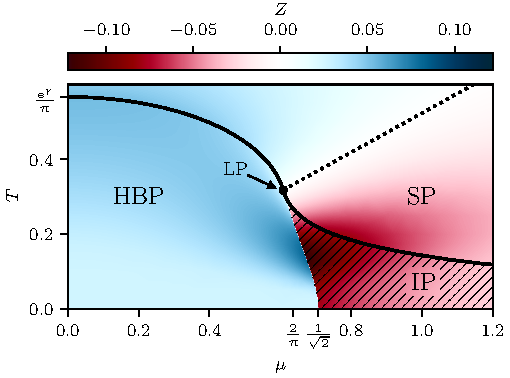
\includegraphics[width=\subcaptionFigureWidth]{gn/figures/stab_pd.pdf} % left figure
		\captionsetup{width=\subcaptionFigureWidth}%
		\caption{%
			The bosonic wave-function renormalization $\zwave{\sminhom ( \mu, T )}{\mu}{T}$ (heat map), line of vanishing wave-function renormalization ${Z ( \sminhom ( \mu, T ), \mu, T ) = 0}$ (thick black dashed line), and the line of vanishing bosonic two-point function ${\gtwovar{\sminhom ( \mu, T )}{\mu}{T}{\qmin} = 0}$ (thick, black solid line) in the $\mu$-$T$-plane. In the region marked by the diagonal hatching using thin black solid lines (bottom-right corner) we find $\gtwovar{\sminhom ( \mu, T )}{\mu}{T}{\qmin} < 0$, \ie{}, the homogeneous minimum is unstable \wrt{} an inhomogeneous perturbation.
			\fromFig{9}{Koenigstein:2021llr}
		}
		\label{fig:pd_stability}
	}
	{\fullWidthTwoColumnFigureSpacing}
	{%
		\vspace{.44cm}
		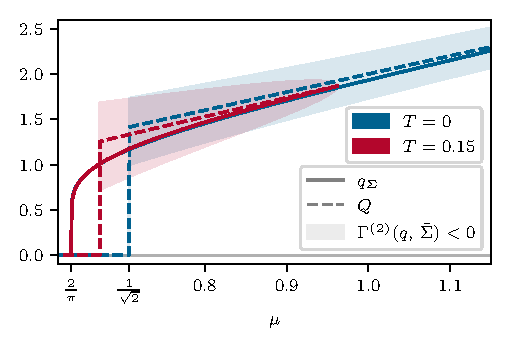
\includegraphics[width=\subcaptionFigureWidth]{gn/figures/q_stab_vs_min.pdf} % Right figure
		\captionsetup{width=\subcaptionFigureWidth}%
		\caption{%
			The minimum of the bosonic two-point function $\qmin ( \mu )$ and the dominating wave vector of the true inhomogeneous condensate $\qs ( \mu )$ as a function of the chemical potential at constant temperatures $T/\snull \in \{ 0.0, 0.15 \}$.
				The colored regions mark the range of momenta $q$, where $\gtwovar{\sminhom ( \mu, T )}{\mu}{T}{q} < 0$.
			\fromFig{10}{Koenigstein:2021llr}
		}%
		\label{fig:stability_wavevector_vs_condensate_wavevector_mu_scan}
		%\vspace{1cm}
	}%
Nonetheless, at the phase boundary of the \gls{hbp} and \gls{ip} the amplitude of the inhomogeneous condensate is large and the inhomogeneous condensate almost oscillates between the values of the homogeneous minima, \ie{}, between $\pm \sminhom(\mu, T)$, \cf{}\ \cref{fig:inhomogeneous_condensate}.
As soon as one crosses the first-order phase transition and needs to switch to one of these minima as the formal correct expansion point, the initial assumption of the stability analysis of small perturbations about the expansion point is violated and one finds a deviation from the exact result.

The additional color map in \cref{fig:pd_stability} shows the value of the wave-function renormalization $\zwave{\shom}{\mu}{T}$, \cref{eq:wave-function_renormalization_definition}, evaluated at the true homogeneous minimum ${\shom = \sminhom ( \mu, T )}$.
It is calculated numerically using the appropriate formulae from App. B of \ccite{Koenigstein:2021llr}.

We also cross-checked that these results coincide with results, which are obtained by a numeric evaluation of the $q$-derivatives of $\gtwo$ in \cref{eq:wave-function_renormalization_definition}.
In the \gls{sp} the wave-function renormalization is given by 
\begin{align}
	\zwave{0}{\mu}{T} = - \frac{1}{8 \uppi} \frac{1}{T^2} \, \mathrm{DLi}_{2} \big( \tfrac{\mu}{T} \big) \, ,	\label{eq:z_0_mu_t}
\end{align}
according to Eq.~(B3) of \ccite{Koenigstein:2021llr}, which entails that the ${(Z=0)}$-line  is given by ${z_{2,1}\simeq1.910}$ from \cref{eq:DLi2Zero1}.
It therefore coincides with the $(\alpha_4=0)$-line from \cref{subsec:GNGL}.
This is well known in the context of the \ggla{} and is encountered frequently in the study of inhomogeneous phases in different models.
It implies that the locations of the \gls{lp} of the inhomogeneous phase and of the \cp{} of the homogeneous phase coincide, see, \eg{}, \ccite{Nickel:2009ke,Abuki:2011pf,Buballa:2014tba} for details.

It is immediately clear that a negative $\zwave{\sminhom ( \mu, T )}{\mu}{T}$ can only be an indication that an inhomogeneous perturbation might lower the action, because negative curvature of $\gtwo$ at ${q = 0}$ does not guarantee that the function has a root.
This scenario is found in the region between the $(Z=0)$-line and the \gls{sp}$\pbArrow$\gls{ip} phase boundary right of the \gls{lp}, where the wave-function renormalization is negative, but the spatially homogeneous ground state is stable.

\FloatBarrier
\paragraph{Regions with $Z<0$: Moat/Lifshitz regimes}\phantomsection\label{paragraph:moat}\mbox{}\\%
We have already encountered such regions with $Z<0$ in \cref{subsec:inhomoLiterature} as an indicator/precursor for inhomogeneous phases in the context of the \frg{} \qcd{} computations of \nbccite{Fu:2019hdw}, \cf{} \cref{fig:fuQCDpd} and specifically \cref{fig:qcdZphis}.

Regions with $Z<0$ and the corresponding modified dispersion relation for bosons are discussed in \ccite{Rennecke:2021ovl,Pisarski:2020gkx,Pisarski:2021qof, Pisarski:2020dnx} and referred to as moat and Lifshitz regimes.
Moat or Lifshitz regimes are regions of negative wave-function renormalization, which signals a dispersion relation with a minimum at a non-zero momentum~\cite{Rennecke:2021ovl,Pisarski:2021qof, Pisarski:2020gkx,Pisarski:2020dnx}. The expression moat regime~\cite{Pisarski:2021qof,Rennecke:2021ovl} goes back to the dispersion relations encountered in these phases, \cf{}\ \cref{fig:gamma2_compare_2}, resembling the  deep, broad ditch \dash{} the moat \dash{} in front of a castle wall.
	
Regions of inhomogeneous phases can be included in such moat regimes, like in the present study, but they do not have to be present since $Z<0$ is not a necessary condition for instability of the homogeneous phase in favor of inhomogeneous condensation.
Other exotic phases of matter, like a quantum spin liquid~\cite{Pisarski:2020dnx}, might be possible and energetically preferred over a typical homogeneous static ground state in the moat regime \dash{} if the particle content and space-time dimensionality of the model is more involved.

In summary, an inhomogeneous field configuration with momentum $q$ that lowers the effective action can only be indirectly detected in the present analysis, when $\gtwovar{\sminhom ( \mu, T )}{\mu}{T}{q} < 0$ and ${\sminhom ( \mu, T ) = 0}$, which corresponds to the hatched region (bottom, right) in \cref{fig:pd_stability}.
The fact that ${\sminhom ( \mu, T ) = 0}$ is required in the present context to find $\gtwovar{\sminhom ( \mu, T )}{\mu}{T}{q} < 0$ is an \aposteriori{} observation rather than an \apriori{} requirement and is related to the potential barrier discussed in the previous \cref{subsubsec:momentum_structure}.

\subsubsection{The wave vector of the inhomogeneous perturbation and the wave vector of the true inhomogeneous condensate}
\label{subsubsec:wavevector}
Even though the stability analysis is expected to work only for very small perturbations about a vanishing homogeneous condensate, we found that it even correctly predicts inhomogeneous condensation at points to the right of the homogeneous first-order phase transition at extremely small temperatures which are far away from the second-order \gls{sp}$\pbArrow$\gls{ip} phase transition line.
At these points one still uses the appropriate expansion point ${\sminhom ( \mu, T ) = 0}$, but the perturbations are no longer small and the true condensate has a spectrum of wave vectors instead of a single frequency/wave vector, \cf{}\ \cref{fig:inhomogeneous_condensate}.
	
One might thus wonder, if the single wave vector $\qmin$ at the phase transition line actually matches the wave vector of the true solution, \ie{}, the dominating wave vector of the Jacobi elliptic functions.
Therefore, we compare the dominating wave vector of the correct inhomogeneous condensate minimizing the effective action 
\begin{equation}
	\qs \equiv \mathrm{argmax}_q \, \tilde{\smin} ( \mu, T, q )
\end{equation}
with the wave vector that minimizes the two-point function $\qmin$ as defined in \cref{eq:qmin}.
While $\qmin$ is the direction of the largest curvature of the action at the saddle-point, it does not necessarily coincide with $\qs$.
In \cref{fig:stability_wavevector_vs_condensate_wavevector_mu_scan} these two quantities  are plotted for two different temperatures.
At ${T = 0}$, $\qmin$ approaches $\qs$ for increasing chemical potential\footnote{Plots similar to \cref{fig:stability_wavevector_vs_condensate_wavevector_mu_scan} of the wave vector of some inhomogeneous condensate plotted over baryon density (chemical potential), can be found in, \eg{}, Fig.~2 of \ccite{Dautry:1979bk}, Fig.~2 of \ccite{Kutschera:1989yz}, Figs.~6 \& 7 of \ccite{Kutschera:1990xk}.} and at ${T/\snull = 0.15}$ the two momenta match at the phase boundary.
This is expected as the amplitude of the inhomogeneous condensate $\smin ( \mu, T, \ex )$ at this point is infinitesimal and therefore the stability analysis becomes exact.
At small chemical potential \dash{} as already discussed before \dash{} the stability analysis does not detect an inhomogeneous phase unless ${\sminhom ( \mu, T ) = 0}$ and thus fails left of the homogeneous first-order phase transition.
At intermediate chemical potential, $\qmin$ and $\qs$ do not agree.
However, $\qs$ is within the interval where $\gtwo < 0$ is predicted by the stability analysis, which means that the latter at least captures the dominating wave vectors.

\customWidthFigure%
	[!t]%
	{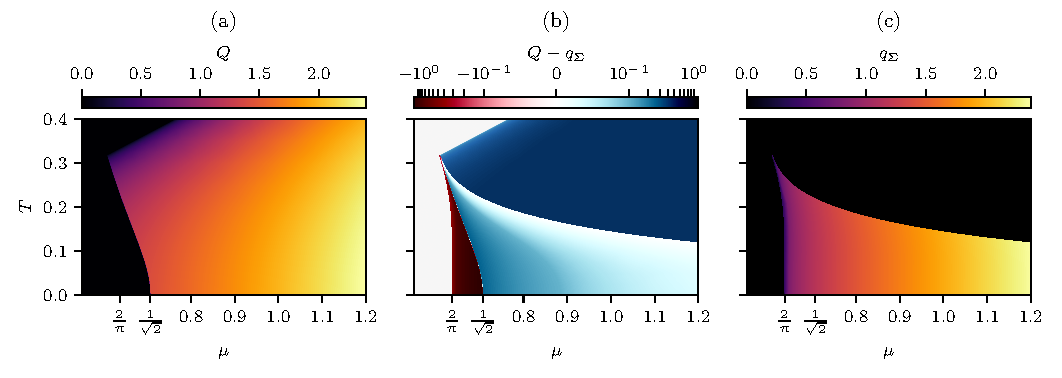
\includegraphics[width=\fullWidthFigureWidth]{gn/figures/q_stab_vs_min_muT.pdf}}% Graphics
	[fig:q_stab_vs_min_muT_qmin,fig:q_stab_vs_min_muT_delta,fig:q_stab_vs_min_muT_qs]% Sublabels
	{%
		Wave vector  $\qmin$  predicted by the stability analysis in \subref{fig:q_stab_vs_min_muT_qmin}, dominating wave vector of the reference solution $\qs$ in \subref{fig:q_stab_vs_min_muT_qs}, and their difference $\qmin-\qs$ in \subref{fig:q_stab_vs_min_muT_delta} in the $(\mu,T)$-plane.
		Note that the colormap in \subref{fig:q_stab_vs_min_muT_delta} is linear around $0$ and logarithmic for values $|(\qmin-\qs)/\snull|>0.1$.
		\fromFig{11}{Koenigstein:2021llr}
	}%Caption
	{fig:stability_wavevector_vs_condensate_wavevector_mu_T}%Label

In \cref{fig:stability_wavevector_vs_condensate_wavevector_mu_T} we again compare $\qmin$ and $\qs$.
This time we plot $\qmin$, $\qmin - \qs$, and $\qs$ in the $\mu$-$T$-plane using different color maps.
The previously discussed trend extends to the whole temperature range.
The difference $\qmin - \qs$ approaches zero close to the \gls{ip}$\pbArrow$\gls{sp} boundary and its magnitude is the largest close to the \gls{hbp}$\pbArrow$\gls{ip} boundary, where $\qmin$ is zero (because the stability analysis is ill-conditioned) and $\qs$ is minimal.
On the other hand, $\qmin$ is also non-zero in the region of $Z < 0$ above the phase transition line, but does not correspond to an inhomogeneous perturbation that lowers the action, since $\gtwo$ is manifestly positive.
We want to emphasize that this does not mark a failure of the employed method, but is rather just an effect of the negative wave-function renormalization $Z$.
A discussion similar to our elaboration on \cref{fig:stability_wavevector_vs_condensate_wavevector_mu_T} can be found in a different context in \ccite{Nakano:2004cd}.\clearpage

\subsubsection{The bosonic wave-function renormalization}
\label{subsubsec:wave-function renormalization}
\fullWidthTwoColumnFigures%
	[!t] % Placement
	{%
		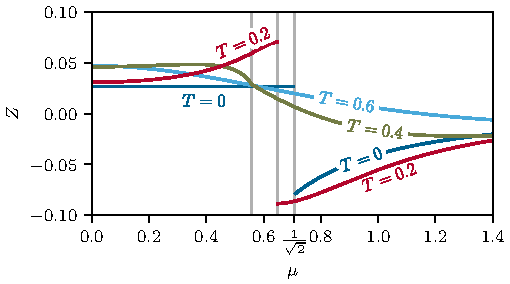
\includegraphics[width=\subcaptionFigureWidth]{gn/figures/Z_slice_0.pdf} % left figure
		\captionsetup{width=\subcaptionFigureWidth}%
		\caption{%
			The bosonic wave-function renormalization $\zwave{\shom}{\mu}{T}$ as a function of the chemical potential at fixed temperatures ${T \in \{0.0, 0.2, 0.4, 0.6 \}}$ evaluated at the homogeneous minimum ${\shom = \sminhom ( \mu, T )}$.
			\fromFig{12}{Koenigstein:2021llr}
		}
		\label{fig:Z_slice_0}
	}
	{\fullWidthTwoColumnFigureSpacing}
	{%
		%\vspace{.44cm}
		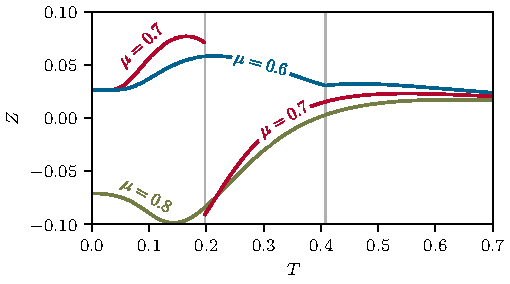
\includegraphics[width=\subcaptionFigureWidth]{gn/figures/Z_slice_1.pdf} % Right figure
		\captionsetup{width=\subcaptionFigureWidth}%
		\caption{%
			The bosonic wave-function renormalization $\zwave{\shom}{\mu}{T}$ as a function of temperature at fixed chemical potentials ${\mu \in \{ 0.55, 0.65, 0.75 \}}$ evaluated at the homogeneous minimum ${\shom = \sminhom ( \mu, T )}$.
			\fromFig{13}{Koenigstein:2021llr}
		}%
		\label{fig:Z_slice_1}
		%\vspace{1cm}
	}%
	
Before closing our discussion of this subsection, we shortly return to our results for the bosonic wave-function renormalization and their implications.

In \cref{fig:pd_stability} the bosonic wave-function renormalization $\zwave{\sminhom ( \mu, T )}{\mu}{T}$ was already presented in the entire $\mu$-$T$-plane.
We stress again that negative values of $Z$ are not a sufficient or even necessary criterion for instabilities of the homogeneous phase.
However, in regions of the phase diagram where the stability analysis is expected to work, \ie{}, regions with ${\sminhom(\mu,T)=0}$, a negative wave-function renormalization presents as a strong indicator for an inhomogeneous phase.
In regions where $\gtwo(q)$ is dominated by low-momentum contributions \dash{} \ie{}, around the \cp{}/\lp{} \dash{} $Z<0$ is a necessary condition for an inhomogeneous phase if contributions of ${\order(q^6)}$ to $\gtwo(q)$ can be neglected, \cf{} the following discussion of the \ggla{} in \cref{subsec:GNggl}.

Apart from this, one can learn a lot from the values of the wave-function renormalization alone.	
In a first rather rough approximation, we can use $Z$ as a measure for the importance of bosonic quantum fluctuations, because it accompanies the trivial quadratic momentum-dependence of the bosonic field in the action \dash{} the kinetic term \dash{} which drives fluctuations.
Inspecting the classical \gls{uv} action of the \gls{gn} model, we find that it lacks by construction a term like $\frac{Z}{2} \, ( \partial_\mu \phi )^2$ \dash{} which is included in the \gnym{} with $Z=1$ \dash{} and also all other bosonic higher-order derivative terms, which could partially be associated to the higher-order Taylor coefficients/moments of $\gtwo$ in momentum space.
Hence, in the classical action of the \gls{gn} model all these coefficients are initially zero, because there are no bosonic fluctuations in the \gls{uv} \dash{} there are only non-interacting fermions \dash{} and $\phi$ is only introduced as an auxiliary field.
However, by integrating out all fermionic quantum fluctuations and interactions one finds that the system gets strongly coupled and anti-fermion-fermion pairs are bosonized and eventually condense, if the external energy scales ($\mu$ and/or $T$) are not too large~\cite{Wolff:1985av,Harrington:1974tf,Dashen:1974xz}.
Ultimately, also all of the bosonic derivative couplings are generated by integrating out the fermion fluctuations, as can be seen from our results for $Z$ and $\gtwo$.
From an \gls{frg} perspective this is a rather natural finding, see \ccite{Dupuis:2020fhh} and references therein.
Though, the generation of all these bosonic kinetic couplings actually implies that the system tends to drive bosonic quantum fluctuations by itself, which is only hindered by the artificially suppression of the infinite-$N$ limit.
Therefore, one might conclude that our results for the bosonic wave-function renormalization (and the bosonic two-point function) in the infinite-$N$ limit may \dash{} at least to some extent \dash{} predict the insufficiency of the mean-field approximation at finite $N$. 
In consequence one might state, that at least in those areas of the phase diagram, where the bosonic wave-function renormalization significantly deviates from zero and rapidly changes its value (and sign) with $\mu$ and $T$, bosonic quantum fluctuations will play an important role, if the infinite-$N$ approximation is relaxed and calculations are performed at finite $N$.
Interestingly, such values are indeed observed, especially close to the first-order phase transition and right below the \gls{lp}.
This is actually expected, since in these regions correlation lengths usually diverge and fluctuations of all orders become relevant.

To better visualize the behavior of $Z$, we additionally plot slices through the color map of \cref{fig:pd_stability} in a way to cover all interesting regions of the phase diagram.
In \cref{fig:Z_slice_0,fig:Z_slice_1} we can observe that the wave-function renormalization increases (decreases) close to the phase transition line\footnote{Except for ${T=0}$, where $\zwave{\sminhom(\mu,0)}{\mu}{0}$ is independent of $\mu$ for $\sminhom(\mu,0)^2>\mu^2 \Leftrightarrow \mu < \tfrac{1}{\sqrt{2}}$, see Eq.~(B5) of \nbccite{Koenigstein:2021llr}. This is a notion of the silver blaze property.} and then jumps from positive to negative values at the phase transition.
The region of drastically rising $Z$ is exactly the region adjacent to the first-order phase transition, where the stability analysis fails.
Thus, it seems as if the wave-function renormalization already signals that fluctuations and gradient driven bosonic field configurations are of great importance in this region.

\subsection{Generalized Ginzburg-Landau analysis}\label{subsec:GNggl}
\begin{disclaimer}
	This subsection is not based on \ccite{Koenigstein:2021llr} and the discussion is original to this work.
	However the presented results are basically just a projection of the results~\cite{Abuki:2011pf} of H. Abuki \etal{} into the $\mu$-$T$-plane using the expressions of \cref{subsec:GNGL,app:Vmedf1Series}.
	In that sense the presented results are just a comparison of existing literature results.
	
	The results for this \ggla{} of the inhomogeneous phase diagram took only a few minutes to compute on an \intel{} with the \WAM{} notebook~\cite{Steil:2023GNnotebook}.
\end{disclaimer}
In this subsection we want to briefly introduce the \acrrepeat{ggl} analysis as another indirect method to study inhomogeneous phases.
To this end we will follow \nbccite{Abuki:2011pf} but additional details can be found in \ccite{\gglRefs} and \nbccite{Steil:2020ggl}.\bigskip

The \ggla{} can be seen as an extension of the conventional \gla{} outlined in \cref{subsec:GNGL}.
The idea is to expand the effective potential or equivalently the effective action in a gradient expansion. 
Up to sixth-order such an expansion for a model like the \gn{} model reads,
\begin{align}
	\VeffFArgs{\muT;\smin (\ex )}\equiv\langle\omega[\muT;\smin (\ex )]\rangle_{\scriptscriptstyle{\mathrm{WS}}} \label{eq:Vggl}
\end{align}\clearpage
\customWidthFigure%
	[!t]%
	{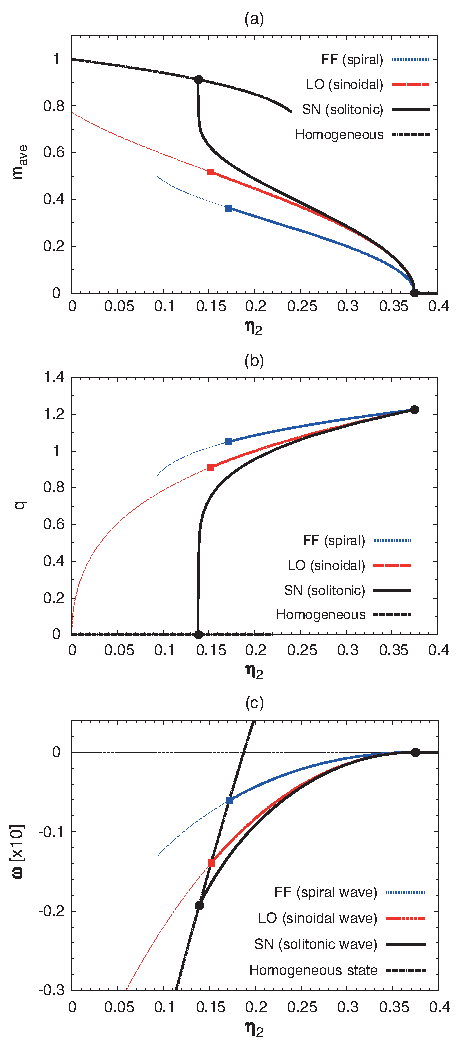
\includegraphics[width=7.5cm]{gn/figures/PhysRevD.85.074002Fig4.pdf}}% Graphics
	[fig:abukiM,fig:abukiq,fig:abukio]% Sublabels
	{%
		Average mass $m_\mathrm{ave}\equiv (\langle \smin (\ex )^2\rangle_{\scriptscriptstyle{\mathrm{WS}}})^{1/2}$ in \subref{fig:abukiM}, wave vector $q$ in \subref{fig:abukiq}, and associated energy $\omega\equiv \VeffFArgs{\muT;\smin (\ex )}$ in \subref{fig:abukio} for various inhomogeneous modulations as a function of $\eta_2^\mathrm{A}$. Note that H. Abuki \etal{} use a different convention for the pre-factors of their \ggl{} coefficients in Eq.~(2) of \ccite{Abuki:2011pf} and thus $\eta_2=\frac{4}{3}\eta_2^\mathrm{A}$.
		\fromFig{4}{Abuki:2011pf}
		\ccbysaLicense{H. Abuki}
	}%Caption
	{fig:abuki}%Label
\clearpage
as the volume average over the Wigner-Seitz cell of the generalized \gl{} functional
\begin{align}
\omega[\muT;\smin (\ex )]&\equiv \alpha_2(\muT) \smin (\ex )^2 +\alpha_4(\muT) \ \big(\smin (\ex )^4 + (\grad \smin (\ex ))^2\big)\,+\notag\\[.2em]
&\qquad\qquad +\alpha_6(\muT) \big(\smin (\ex )^6 + 5\smin (\ex )^2(\grad \smin (\ex ))^2+\tfrac{1}{2}(\Delta \smin (\ex ) )^2\big)\,
\label{eq:omegaggl}
\end{align}
according to Eqs.~(2) and (6) in \ccite{Abuki:2011pf}.
When rescaling all quantities appropriately with $\alpha_6$ and setting the scale with $|\alpha_2|$, the \rhs{} of \cref{eq:omegaggl} has only $\eta_2\equiv \alpha_2 \,\alpha_6/\alpha_4^2$ from \cref{eq:GLeta2} as a parameter left.
The great advantage of this expansion is that it allows the study of various condensate shapes without the need of any complicated field-theoretical computation.
A condensate shape $\smin (\ex )$ gets inserted into \cref{eq:omegaggl} and with \cref{eq:Vggl} the corresponding energy can be computed just by taking a suitable volume average.
Additionally it is possible to consider Euler-Lagrange equations for $\VeffFArgs{\muT;\smin (\ex )}$ which, when limited to one-dimensional modulations, yield the solitonic solutions \eqref{eq:Msn} of the \gnm{} as a self-consistent solution.
For further details we refer to \ccite{Abuki:2011pf,Steil:2020ggl}.

In \cref{fig:abuki} results for several one-dimensional modulations are shown over $\eta_2$, with the solitonic wave of the \gnm{} as the energetically most favored solution. 
Furthermore $\eta_2=5/27$ ($1/2$)\footnote{
	Note that H. Abuki \etal{} use a different convention for the pre-factors of their \ggl{} coefficients in Eq.~(2) of \nbccite{Abuki:2011pf} and thus $\eta_2=\frac{4}{3}\eta_2^\mathrm{A}$, \ie{},
	the values on the horizontal axis of \cref{fig:abuki} have to be rescaled by a factor $\frac{4}{3}$ to be consistent with the discussion in the text here.
} can be identified as the location of the \gls{hbp}$\pbArrow$\gls{ip} (\gls{ip}$\pbArrow$\gls{sp}) second-order phase transition.
We can use those results with our \gl{} coefficients of \cref{subsec:GNGL} to project the results~\cite{Abuki:2011pf} of H. Abuki \etal{} in terms of $\eta_2$  into the $\mu$-$T$-plane.
The result is shown in \cref{fig:ggl_pd} together with the reference values of \cref{subsec:phenomenology}.
As one might expect from an expansion basically around the restored/trivial solution $\smin (\ex )=0$ the \ggle{} loses predictive power when leaving the vicinity of the \lp{}.
But it should be noted that around the \lp{} it has both qualitative and quantitative predictive power and might be one of the most promising options when it comes to the search of the preferred condensate shape in models, where the solution to this question is not known. 
Which basically includes all models in $d>2$.

We close this discussion by noting, that the stability analysis via the bosonic two-point function, as it is presented in the last \cref{subsec:stability}, goes beyond the \ggle{} discussed here.
The bosonic two-point function \cref{eq:gtwo_renorm} retains its full momentum structure, which makes the stability analysis suited for wave vectors $q$ of all magnitudes without the limitation to small $q$.
Comparing \cref{fig:ggl_pd,fig:q_stab_vs_min_muT_delta} clearly shows the difference in predictive power.
Additionally, $\gtwo$ does not even need to be analytic for all $q$.
This was already pointed out in \ccite{Carignano:2019ivp} and such a non-analyticity can be seen in \cref{fig:gamma2_compare_2} for $T=0$.
It is also the reason, why the stability analysis is still predicting instabilities of the homogeneous condensate correctly for extremely small and even vanishing temperatures.

It should however be noted that there exist several improved versions, see, \eg{}, \ccite{Abuki:2011pf,Abuki:2013pla,Carignano:2017meb}, of the simple expansion up to order six discussed here.\clearpage
\customWidthFigure%
	[t]%
	{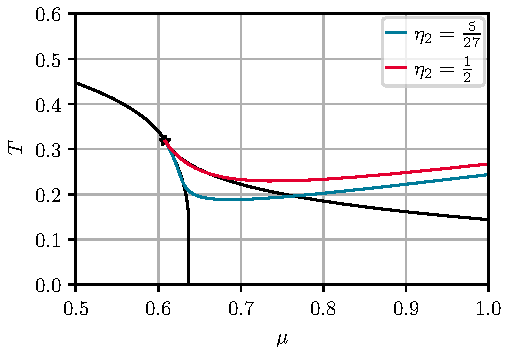
\includegraphics[width=7cm]{gn/figures/ggl_pd.pdf}}% Graphics
	[]% Sublabels
	{%
		Results for the \gls{hbp}$\pbArrow$\gls{ip} and \gls{ip}$\pbArrow$\gls{sp} second-order phase transitions with the \ggla{} ($\eta_2=5/27$ and $\eta_2=1/2$) compared to the reference solution of \cref{fig:analytical_pd}.
	}%Caption
	{fig:ggl_pd}%Label